\begin{surferPage}[A2+- Cusp]{A Cusp ($A_2^{+-}$ Singularity)}
The following equation corresponds to a so-called cusp-singularity:
    \vspace*{-0.4em}
    \begin{center}
      $x^3+y^2-z^2=0.$
    \end{center}
    \vspace*{-0.4em}
    This is the surface variant of a plane cusp which we obtain by cutting the
    surface with an appropriate plane.
    E.g., $z=0$ yields the plane curve with equation $x^3+y^2=0$:
    \vspace*{-0.7em}
    \begin{center}
      \begin{tabular}{c@{\ }c@{\ }c@{\ }c}
        \begin{tabular}{@{}c@{}}
          
\includegraphics[width=1.2cm]{../../common/images/A2pm}
        \end{tabular}
        &
        \begin{tabular}{@{}c@{}}
          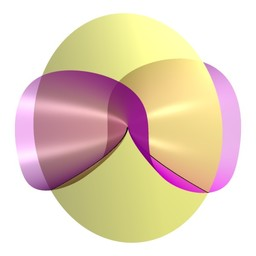
\includegraphics[width=1.2cm]{../../common/images/cuspe_cut}
        \end{tabular}
        &
        \begin{tabular}{@{}c@{}}
          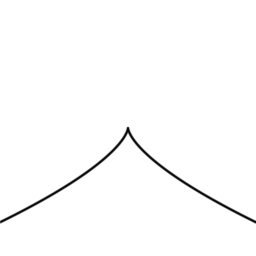
\includegraphics[width=1.2cm]{../../common/images/cuspe_rot}
        \end{tabular}
        &
        \begin{tabular}{@{}c@{}}
          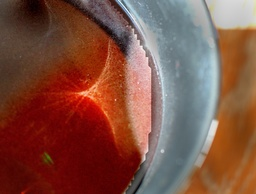
\includegraphics[width=1.4cm]{../../common/images/kuspe_detail_gross_heller}
        \end{tabular}
      \end{tabular}
    \end{center}
    \vspace*{-0.4em}
    A cusp appears naturally when light is reflected in a cup (rightmost picture)! 

    One can deform a singularity of type $A_k^{+-}$ in a way such that 
    $\lfloor\frac{k+1}{2}\rfloor$ double cone - singularities develop without
    increasing the degree of the surface.
    Here, we show the case $k=2$;
    the deformation is as follows:
    \[(1-a)x^3+ax^2+y^2-z^2=0.\]
    For $a=0$ we get a cusp, and for small values $a\neq 0$ a double cone:  
    \vspace*{-0.6em}
    \begin{center}
      \begin{tabular}{@{}c@{\quad}c@{\quad}c@{}}
        \begin{tabular}{@{}c@{}}
          
\includegraphics[width=1.1cm]{../../common/images/A2pm_0}
        \end{tabular}
        &
        \begin{tabular}{@{}c@{}}
          
\includegraphics[width=1.1cm]{../../common/images/A2pm_1}
        \end{tabular}
        &
        \begin{tabular}{@{}c@{}}
          
\includegraphics[width=1.1cm]{../../common/images/A2pm_2}
        \end{tabular}
      \end{tabular}
    \end{center}
 
\end{surferPage}
